\chapter{Einführung} 
%Aufgabenstellung, Problematik und Zielsetzung der Arbeit als Vorausschau (1-2 Seiten)

\section{Einordnung der Arbeit}
Dieser Abschnitt beschreibt die Einordung der Arbeit in den Kontext des 
Projektes.

Ein elektrischer Oszillator ist eine Schaltung, die an seinem Ausgang ein
Signal mit einer bestimmten Frequenz erzeugt.

Für den Bau von elektrischen Ozillatoren gibt es verschiedene Topologien.
Zu den charakterisierenden Eigenschaften von Oszillatoren gehören neben
der Frequenz $f$ des Oszillators, die Frequenzstabilität und das Spektrum des 
Ausgangssignals.

Für ein Spektrum mit kleinen Anteilen von Frequenzen, die nicht die des 
Ausgangssignals sind, können Oszillatoren mit einer Wien-Robinson-Brücke als 
frequenzbestimmendes Element genutzt werden.

Der im Projekt verwendete Wien-Oszillator soll durch eine rauscharme 
Spannungsquelle mit der Betriebsspannung versorgt werden.
Zu den charakterisierenden Eigenschaften von Spannungquellen gehören neben der
Ausgangsspannung, das Verhältnis der Eingangsspannungsänderung zur 
Ausgangsspanngsänderung (eng.\ power supply rejection ratio — PSRR),
das Verhältnis der Änderung der Ausgangsspannung zur Änderung der Ausgangslast
(eng.\ load regulation) und das Spaktrum der Ausgangsspannung.

In der Anwendung als Spannungsversorgung eines Wien-Oszillators ist die 
Ausgangslast konstant. Die Lastregelungsfähigkeit hat also eine untergeordnete
Bedeutung. Der Oszillator soll über ein Labornetzteil mit der 
Versorgungsspannung versorgt werden. Somit können Einflüsse der 
Veränderung der Eingangsspannung minimiert werden. 

\section{Grundlagen Linearspannungsregler}
Dieser Abschnitt beschreibt die Funktion eines Linearreglers allgemein.

Eine elektrische Schaltung benötigt in der Regel eine konstante 
Versorgungsspannung um ihre Funktion zu erfüllen.
Eine Änderung der Spannung kann zur Verschiebung von Arbeitspunkten und damit
zu einer Veränderung des Verhaltens der Schaltung führen.

Um die Versorgungsspannung einer Schaltung konstant zu halten werden 
verschiedene Ansätze verwendet:

\begin{itemize}
  \item chemische Konstantspannungsquellen
  \item DCDC-Konverter
  \item Linearspannungsregler
\end{itemize}

Chemische Konstantspannungsquellen erzeugen eine Ausgangsspannung mit einer 
hohen spektralen Reinheit, da diese ihre Ausgangsspannung von anderen 
Störeinflüssen getrennt aus einer chemischen Reaktion erzeugen.
Nachteilig bei der Benutzung chemischer Quellen ist der Wartungsaufwand, der

DCDC-Konverter haben in der Regel einen hohen Wirkungsgrad (bis 
98\%~\cite[Industr.com]{Webp:DCDC98}) über einen großen
Eingangsspannungsbereich und können je nach verwendeter Topologie auch 
Ausgangsspannungen größer als die Eingangsspung erzeugen.
Nachteilig ist, dass die Schaltfrequenz der benutzten Schalter im Spektrum der
Ausgangsspannung sichtbar ist und aufwändig gefiltert werden muss.

Linearspannungsregler haben, durch den Verzicht auf schaltende Elemente eine
hohe Spektrale Reinheit der Ausgangsspannung.
Der Wirkungsgrad eines Linearspannungsreglers hängt von der Differenz der 
Eingangsspannung zur Ausgangsspannung ab:
\[\eta = \frac{P_{\rm out}}{P_{\rm in}} \approx \frac{U_{\rm out} 
\cdot I}{U_{\rm in} \cdot I} = \frac{U_{\rm out}}{U_{\rm in}}\]
Ist die Ausgangsspannung der Schaltung nahe an der Eingangsspannung,
so ist der Wirkungsgrad hoch undm mit dem Wirkungsgrad einer 
DCDC-Konverterschaltung vergleichbar. Ist die Ausgangsspannung viel kleiner als die
Eingangsspannung, so ist auch der Wirkungsgrad kleiner.
Die Differenz zwischen Eingangsleistung und Ausgangsleistung geht im 
Spannungregler als Wärme verloren. 

Der Linearspannungsregler besteht sich aus einem aktiven Element, meist ein 
Bipolartransistor oder einem MOSFET, einer Regeleinrichtung und einer 
Spannungsreferenz.
Das aktive Element wird in dieser Schaltung als steuerbarer Widerstand 
eingesetzt.
Die Regeleinrichtung vergleicht die Ausgangsspannung mit der Spannung der 
Spannungsreferenz und erzeugt aus der Differenz dieser Spannungen ein 
Ansteuersignal für das aktive Element.
Die Spannungsreferenz soll die Sollspannung unabhängig von der Eingangsspannung
erzeugen.
Die Abb.~\ref{FIG:LINREG} zeigt ein Beispiel eines Linearreglers mit einem
MOSFET als aktives Element, einem Operationsverstärker als Regler und einer
Z-Diode als Referenzspannungsquelle.

\begin{figure}
  \centering
  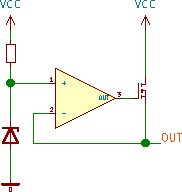
\includegraphics[clip, width=0.33\textwidth]
  {./../common/schaltungen/linearregler/linearregler.pdf}
  \caption{Linearregler}\label{FIG:LINREG}
\end{figure}

\section{Ziel der Arbeit}
Ziel der Arbeit ist es einen Linearregler zu entwerfen, der eine rauscharme
Ausgangsspannung, zur Versorgung eines Wien-Brücken-Oszillators, zur Verfügung
stellt.
Die Parameter der Last sind in der folgenden Tabelle aufgeführt:

\begin{tabularx}{0.9\textwidth}{lrX}
  Parameter&Wert&Einheit\\
  \toprule
  Spannung&$U_{\pm os}\pm 15$&\si{\volt}\\
  Strom&$\overline{i_{\rm os}} = 10$&\si{\ampere}\\
  Ausgangsfrequenz&$f_{\rm os} = 440$&\si{\hertz}\\  
\end{tabularx}

Die Abb.~\ref{FIG:OSZ} zeigt die Oszillatorschaltung.
\begin{figure}
  \centering
  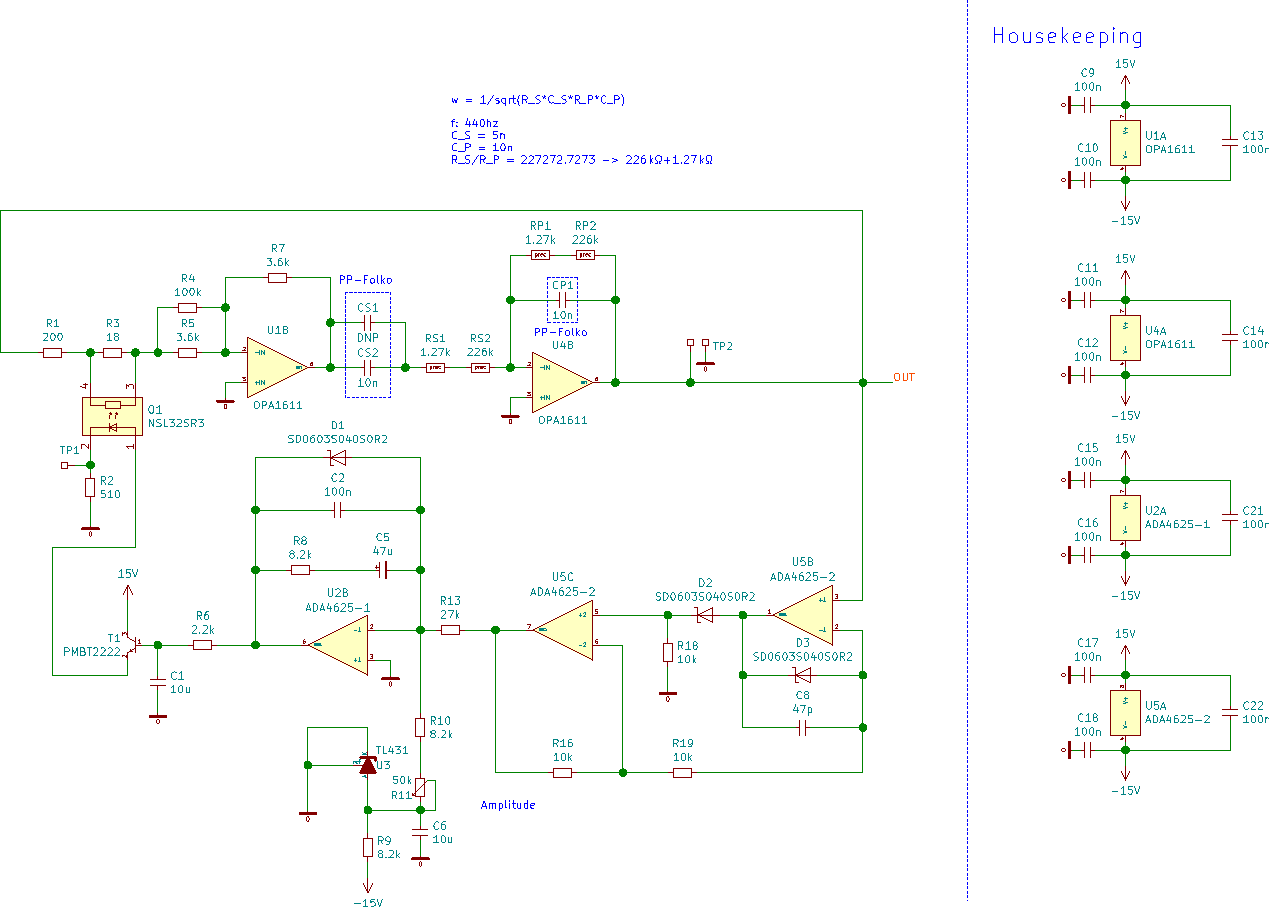
\includegraphics[clip, width=0.9\textwidth]
  {./../common/schaltungen/last.pdf}
  \caption{Linearregler}\label{FIG:OSZ}
\end{figure}

Die Last ist konstant und muss ihrerseits keine weitere Last treiben.

\section{Rauschen}
Unter dem Begriff Rauschen versteht man die nicht systematische veränderungen
eines Signals.
Dieser Abschnitt erläutert die Quellen und die Wirkungen des Rauschens.\\

\textbf{Thermisches Rauschen}

Das thermische Rauschen oder Widerstandsrauschen entsteht aus der thermischen 
Bewegung der Ladungsträger in einem Leiter.
Diese Bewegung erzeugt, in einer aufgrund der Anzahl der Ladungsträger
hohen Rate, positive, wie negative, Spannungs und Stromimpulse. 
Die Abb.:~\ref{FIG:NOISE} zeigt ein solches Rauschsignal.
\begin{figure}
  \centering
  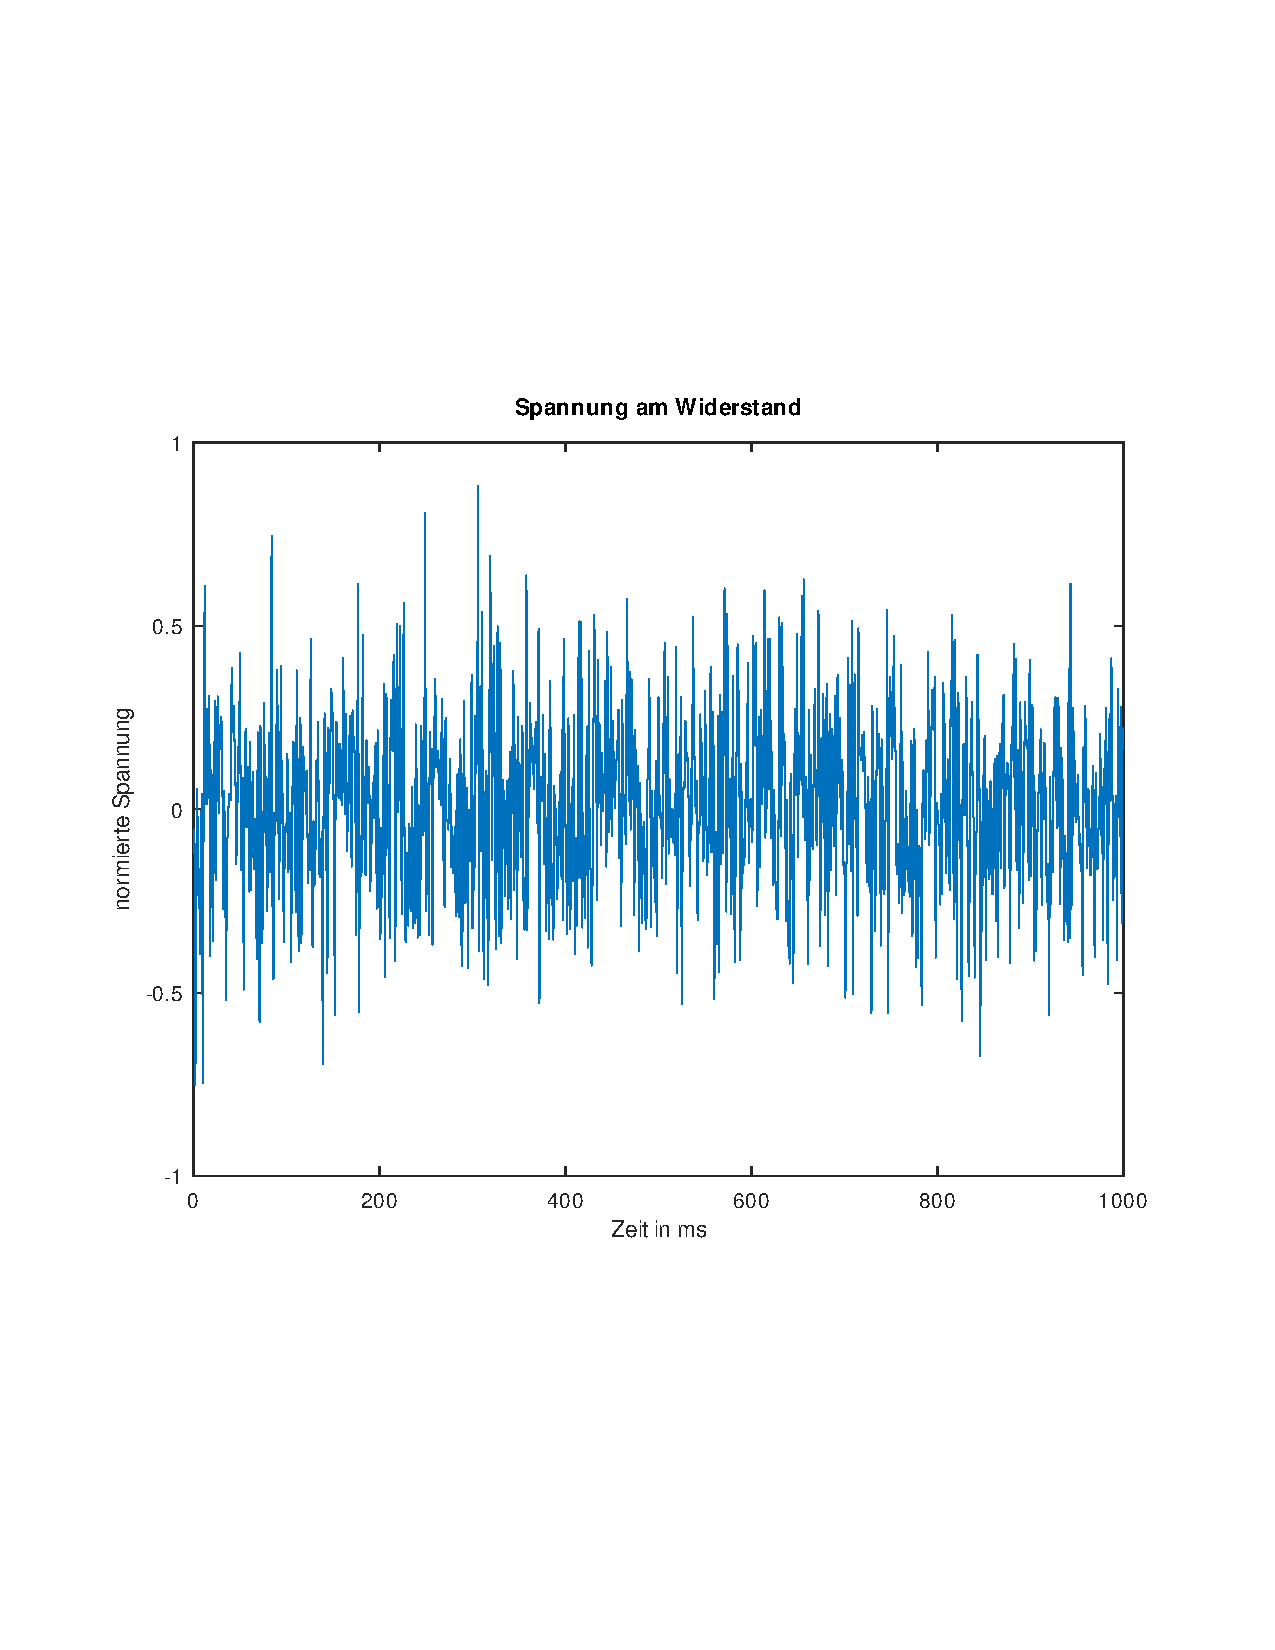
\includegraphics[clip, width=0.49\textwidth]
  {./../common/Simulation/rauschen/spannung.pdf}
  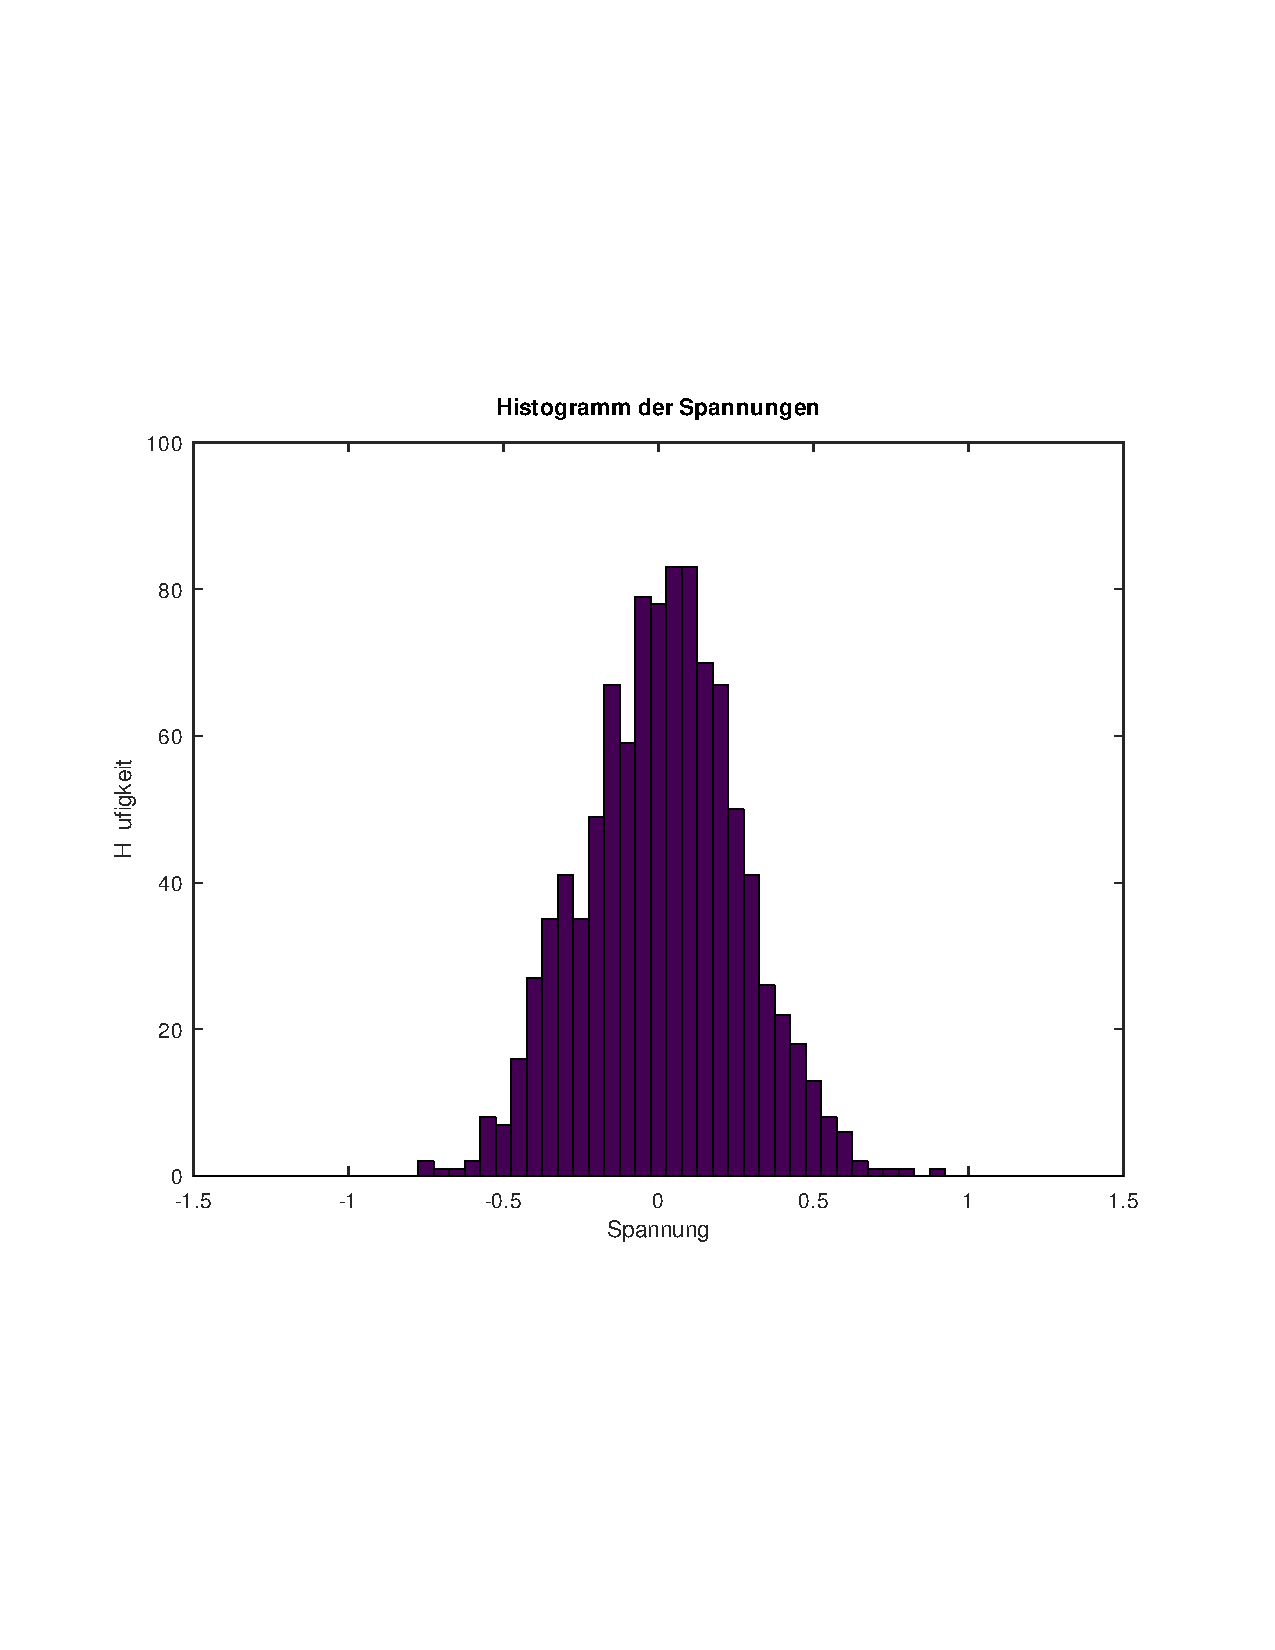
\includegraphics[clip, width=0.49\textwidth]
  {./../common/Simulation/rauschen/haeufigkeit.pdf}
  \caption{Rauschen an einem Widerstand}\label{FIG:NOISE}
\end{figure}
Aufgrund der zufälligen Bewegung ist die spektrale Zusammensetzung der dabei
entstehenden Spannung bis zu einer bestimmten Grenzfrequenz gleichverteilt.
Man spricht daher auch von einem weißen Rauschen.
Die Grenzfrequenz ergibt sich aus Energie der Teilchen geteilt durch das 
planksche Wirkungsquantum:
\[f_{\max} = \frac{k_{\rm B} T}{h}\]
Die Leistung dieses Rauschens ist von der Temperatur des Leiters abhängig und
zu dieser proportional.

\begin{figure}
  \centering
  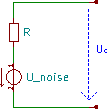
\includegraphics[clip, width=0.49\textwidth]
  {./../common/schaltungen/widerstandsrauschen/widerstandsrauschen.pdf}
  \caption{Rauschen an einem Widerstand}\label{FIG:NOISEESB}
\end{figure}
Für einen Widerstand lässt sich das Ersatzschaltbild aus 
Abb.:~\ref{FIG:NOISEESB} Angeben.
Betrachtet man die Rauschspannung an einem Widerstand 
(vgl. Abb.:~\ref{FIG:NOISE}), so ist diese im zeitlichen Mittel 0.
Der Effektivwert der Leerlaufrauschspannung lässt sich mit der Nyquist-Formel 
und der verfügbaren Bandbreite $\Delta f$ angeben\cite[Nyquist]{Art:NYQUIST}:
\[U_{\rm eff} = \sqrt{4\, k_{\rm B}\, T\, R\, \Delta f}\]
Der Effektivwert des Kurzschlussstroms ergibt sich zu:
\[I_{\rm eff} = \sqrt{\frac{4\,k_{\rm B}\, T\, \Delta f}{R}}\]
Bei Raumtemperatur beträgt der Effektivwert der Rauschspannung an den 
Anschlüssen eines Widerstands von einem \si{\kilo\ohm} also:
\[U_{\rm eff} = 
\sqrt{4\, k_{\rm B}\, 293\,\si{\kelvin}\, 1\,\si{\kilo\ohm} \Delta 
\frac{k_{\rm B} 293\,\si{\kelvin}}{h}} \approx 9.939\,\si{\milli\volt}\]

\textbf{Schrotrauschen}

Muss ein elektrischer Strom eine Potentialbarriere (z. B. verursacht 
durch einen PN Übergang) überwinden, so tun dies die Ladungsträger an der 
Barriere nicht zur selben Zeit. Die Ladungsträger passieren die Barriere
auf unterschiedlichen Pfaden, wodurch die Menge der Ladungsträger im Bereich 
der Barriere schwankt.
Schrotrauschen erfordert das Fließen eines elektrischen Stroms und lässt sich 
mit folgender Gleichung angeben:
\[I_{\rm eff} = \sqrt{2\,I\,e\,\Delta f }\]
Die Spektrale Zusammensetzung des Signals ist wie beim thermischen Rauschen
über den betrachteten Frequenzbereich gleichverteilt.
Auch hier spricht man also von weißem Rauschen.  



\section{Einordnung der Arbeit}
Dieser Abschnitt beschreibt die Einordung der Arbeit in den Kontext des 
Projektes.

Ein elektrischer Oszillator ist eine Schaltung, die an seinem Ausgang ein
Signal mit einer bestimmten Frequenz erzeugt.

Für den Bau von elektrischen Ozillatoren gibt es verschiedene Topologien.
Zu den charakterisierenden Eigenschaften von Oszillatoren gehören neben
der Frequenz $f$ des Oszillators, die Frequenzstabilität und das Spektrum des 
Ausgangssignals.

Für ein Spektrum mit kleinen Anteilen von Frequenzen, die nicht die des 
Ausgangssignals sind, können Oszillatoren mit einer Wien-Robinson-Brücke als 
frequenzbestimmendes Element genutzt werden.

Der im Projekt verwendete Wien-Oszillator soll durch eine rauscharme 
Spannungsquelle mit der Betriebsspannung versorgt werden.
Zu den charakterisierenden Eigenschaften von Spannungquellen gehören neben der
Ausgangsspannung, das Verhältnis der Eingangsspannungsänderung zur 
Ausgangsspanngsänderung (eng.\ power supply rejection ratio — PSRR),
das Verhältnis der Änderung der Ausgangsspannung zur Änderung der Ausgangslast
(eng.\ load regulation) und das Spaktrum der Ausgangsspannung.

In der Anwendung als Spannungsversorgung eines Wien-Oszillators ist die 
Ausgangslast konstant. Die Lastregelungsfähigkeit hat also eine untergeordnete
Bedeutung. Der Oszillator soll über ein Labornetzteil mit der 
Versorgungsspannung versorgt werden. Somit können Einflüsse der 
Veränderung der Eingangsspannung minimiert werden. 

\section{Grundlagen Linearspannungsregler}
Dieser Abschnitt beschreibt die Funktion eines Linearreglers allgemein.

Eine elektrische Schaltung benötigt in der Regel eine konstante 
Versorgungsspannung um ihre Funktion zu erfüllen.
Eine Änderung der Spannung kann zur Verschiebung von Arbeitspunkten und damit
zu einer Veränderung des Verhaltens der Schaltung führen.

Um die Versorgungsspannung einer Schaltung konstant zu halten werden 
verschiedene Ansätze verwendet:

\begin{itemize}
  \item chemische Konstantspannungsquellen
  \item DCDC-Konverter
  \item Linearspannungsregler
\end{itemize}

Chemische Konstantspannungsquellen erzeugen eine Ausgangsspannung mit einer 
hohen spektralen Reinheit, da diese ihre Ausgangsspannung von anderen 
Störeinflüssen getrennt aus einer chemischen Reaktion erzeugen.
Nachteilig bei der Benutzung chemischer Quellen ist der Wartungsaufwand, der

DCDC-Konverter haben in der Regel einen hohen Wirkungsgrad (bis 
98\%~\cite[Industr.com]{Webp:DCDC98}) über einen großen
Eingangsspannungsbereich und können je nach verwendeter Topologie auch 
Ausgangsspannungen größer als die Eingangsspung erzeugen.
Nachteilig ist, dass die Schaltfrequenz der benutzten Schalter im Spektrum der
Ausgangsspannung sichtbar ist und aufwändig gefiltert werden muss.

Linearspannungsregler haben, durch den Verzicht auf schaltende Elemente eine
hohe Spektrale Reinheit der Ausgangsspannung.
Der Wirkungsgrad eines Linearspannungsreglers hängt von der Differenz der 
Eingangsspannung zur Ausgangsspannung ab:
\[\eta = \frac{P_{\rm out}}{P_{\rm in}} \approx \frac{U_{\rm out} 
\cdot I}{U_{\rm in} \cdot I} = \frac{U_{\rm out}}{U_{\rm in}}\]
Ist die Ausgangsspannung der Schaltung nahe an der Eingangsspannung,
so ist der Wirkungsgrad hoch undm mit dem Wirkungsgrad einer 
DCDC-Konverterschaltung vergleichbar. Ist die Ausgangsspannung viel kleiner als die
Eingangsspannung, so ist auch der Wirkungsgrad kleiner.
Die Differenz zwischen Eingangsleistung und Ausgangsleistung geht im 
Spannungregler als Wärme verloren. 

Der Linearspannungsregler besteht sich aus einem aktiven Element, meist ein 
Bipolartransistor oder einem MOSFET, einer Regeleinrichtung und einer 
Spannungsreferenz.
Das aktive Element wird in dieser Schaltung als steuerbarer Widerstand 
eingesetzt.
Die Regeleinrichtung vergleicht die Ausgangsspannung mit der Spannung der 
Spannungsreferenz und erzeugt aus der Differenz dieser Spannungen ein 
Ansteuersignal für das aktive Element.
Die Spannungsreferenz soll die Sollspannung unabhängig von der Eingangsspannung
erzeugen.
Die Abb.~\ref{FIG:LINREG} zeigt ein Beispiel eines Linearreglers mit einem
MOSFET als aktives Element, einem Operationsverstärker als Regler und einer
Z-Diode als Referenzspannungsquelle.

\begin{figure}
  \centering
  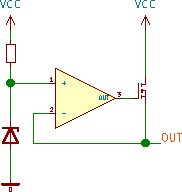
\includegraphics[clip, width=0.33\textwidth]
  {./../common/schaltungen/linearregler/linearregler.pdf}
  \caption{Linearregler}\label{FIG:LINREG}
\end{figure}

\section{Ziel der Arbeit}
Ziel der Arbeit ist es einen Linearregler zu entwerfen, der eine rauscharme
Ausgangsspannung, zur Versorgung eines Wien-Brücken-Oszillators, zur Verfügung
stellt.
Die Parameter der Last sind in der folgenden Tabelle aufgeführt:

\begin{tabularx}{0.9\textwidth}{lrX}
  Parameter&Wert&Einheit\\
  \toprule
  Spannung&$U_{\pm os}\pm 15$&\si{\volt}\\
  Strom&$\overline{i_{\rm os}} = 10$&\si{\ampere}\\
  Ausgangsfrequenz&$f_{\rm os} = 440$&\si{\hertz}\\  
\end{tabularx}

Die Abb.~\ref{FIG:OSZ} zeigt die Oszillatorschaltung.
\begin{figure}
  \centering
  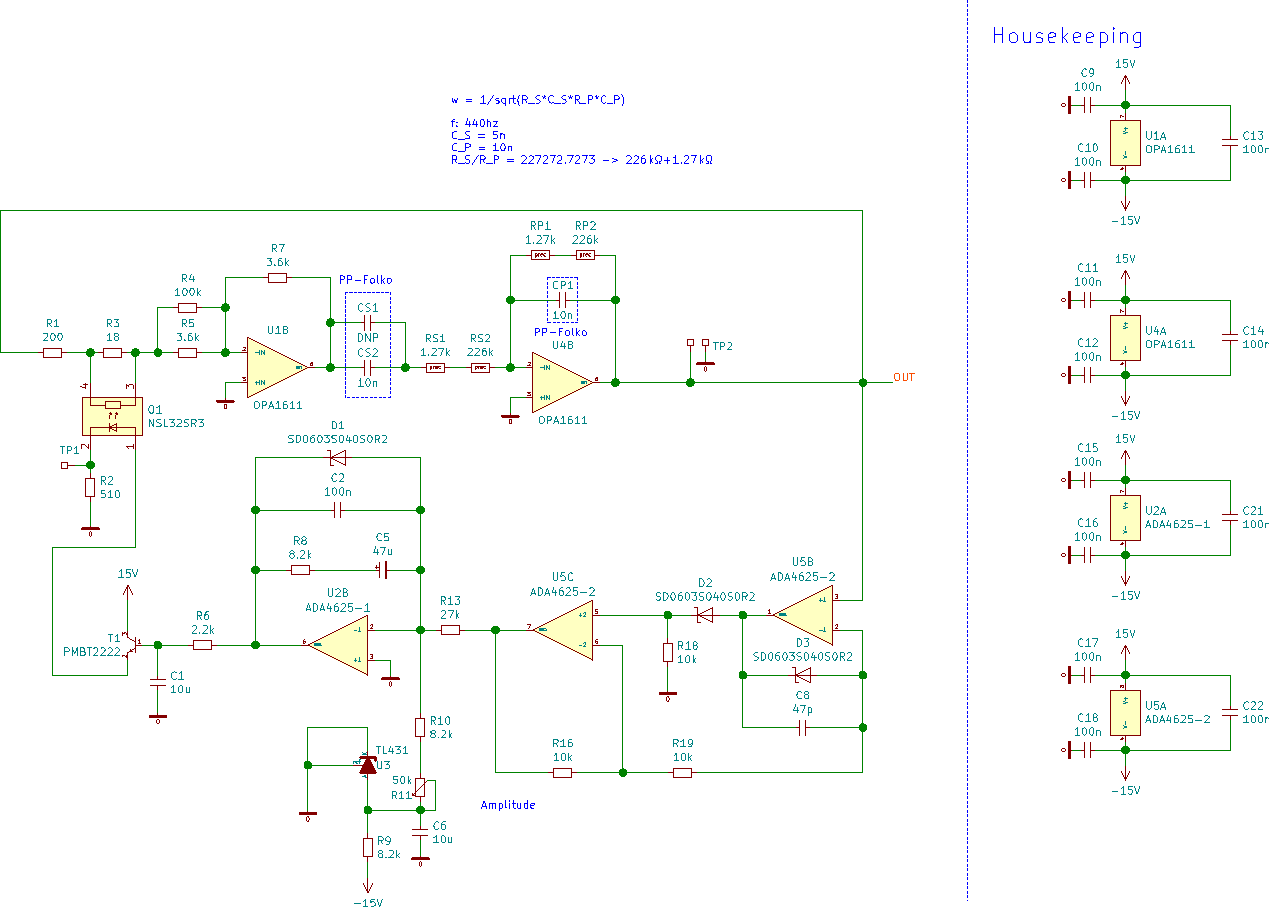
\includegraphics[clip, width=0.9\textwidth]
  {./../common/schaltungen/last.pdf}
  \caption{Linearregler}\label{FIG:OSZ}
\end{figure}

Die Last ist konstant und muss ihrerseits keine weitere Last treiben.

\section{Rauschen}
Unter dem Begriff Rauschen versteht man die nicht systematische veränderungen
eines Signals.
Dieser Abschnitt erläutert die Quellen und die Wirkungen des Rauschens.\\

\textbf{Thermisches Rauschen}

Das thermische Rauschen oder Widerstandsrauschen entsteht aus der thermischen 
Bewegung der Ladungsträger in einem Leiter.
Diese Bewegung erzeugt, in einer aufgrund der Anzahl der Ladungsträger
hohen Rate, positive, wie negative, Spannungs und Stromimpulse. 
Die Abb.:~\ref{FIG:NOISE} zeigt ein solches Rauschsignal.
\begin{figure}
  \centering
  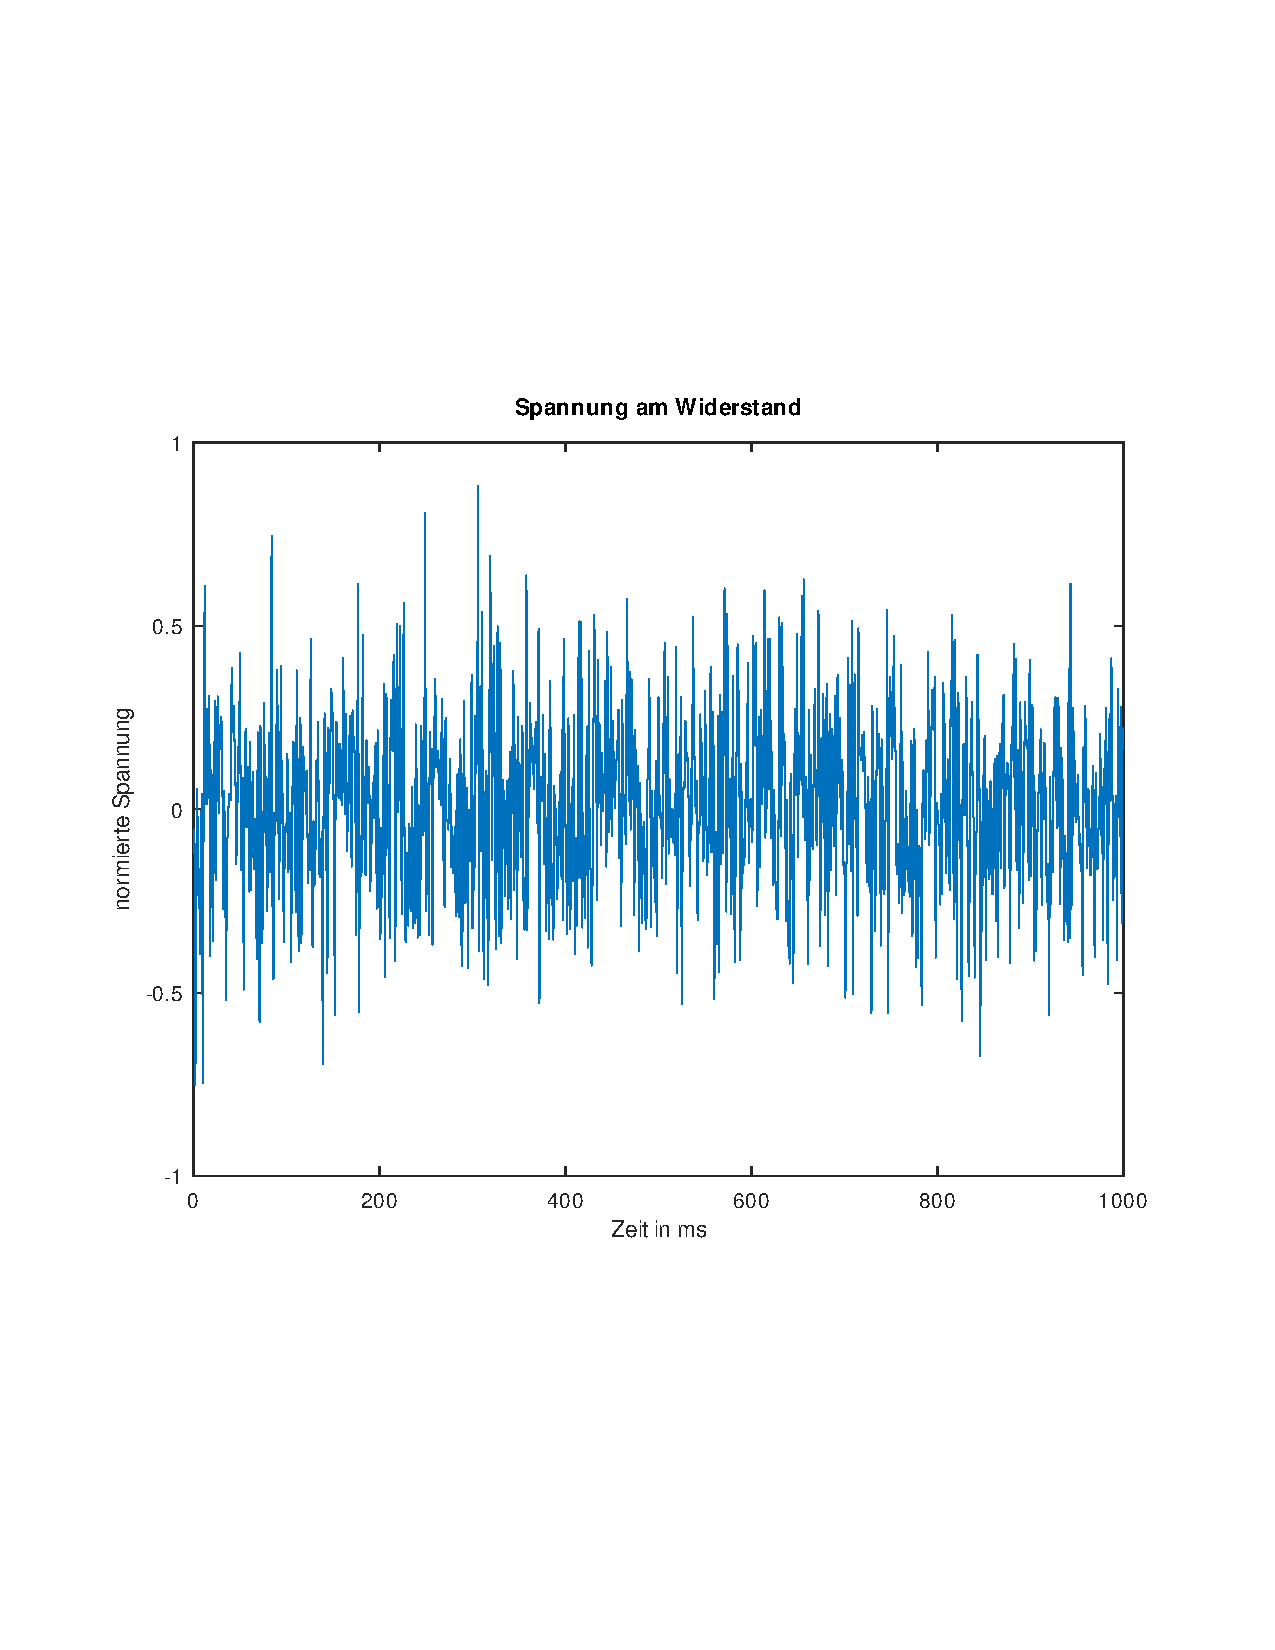
\includegraphics[clip, width=0.49\textwidth]
  {./../common/Simulation/rauschen/spannung.pdf}
  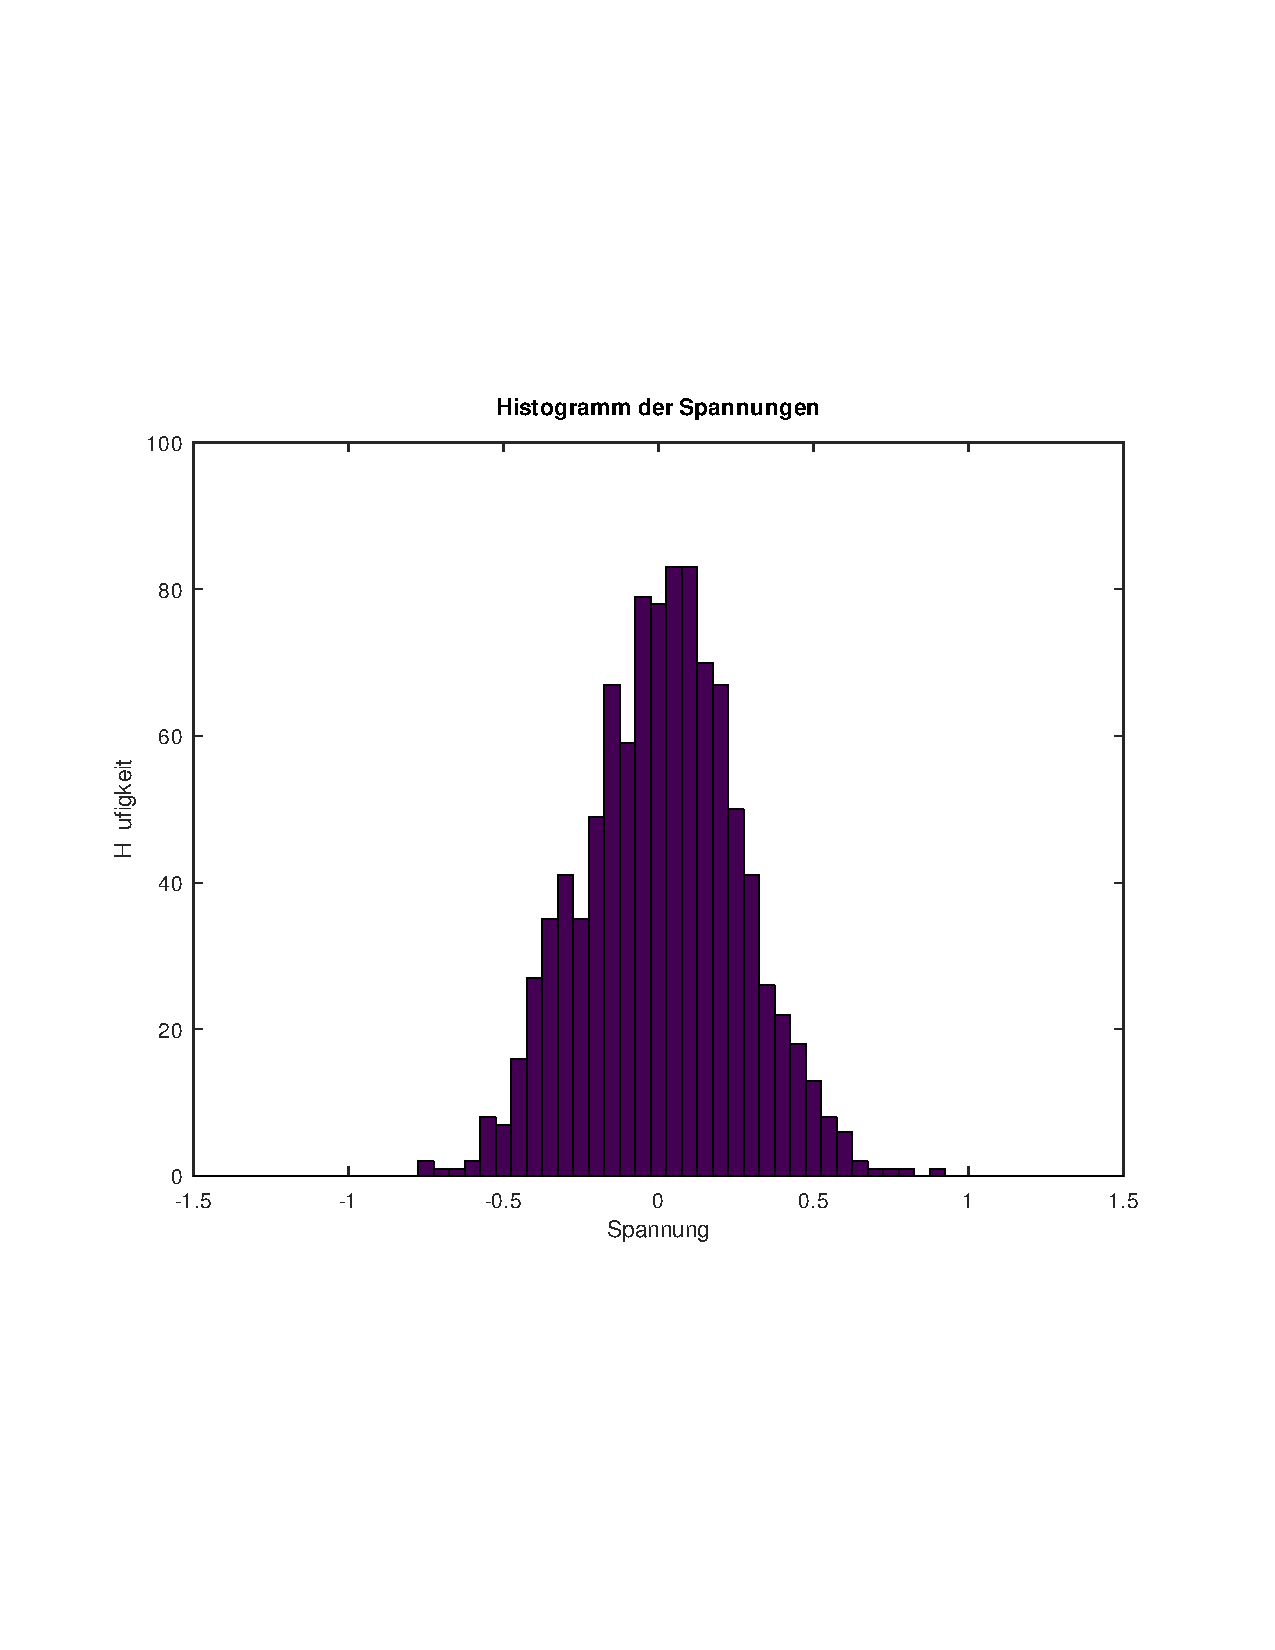
\includegraphics[clip, width=0.49\textwidth]
  {./../common/Simulation/rauschen/haeufigkeit.pdf}
  \caption{Rauschen an einem Widerstand}\label{FIG:NOISE}
\end{figure}
Aufgrund der zufälligen Bewegung ist die spektrale Zusammensetzung der dabei
entstehenden Spannung bis zu einer bestimmten Grenzfrequenz gleichverteilt.
Man spricht daher auch von einem weißen Rauschen.
Die Grenzfrequenz ergibt sich aus Energie der Teilchen geteilt durch das 
planksche Wirkungsquantum:
\[f_{\max} = \frac{k_{\rm B} T}{h}\]
Die Leistung dieses Rauschens ist von der Temperatur des Leiters abhängig und
zu dieser proportional.

\begin{figure}
  \centering
  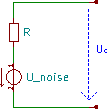
\includegraphics[clip, width=0.49\textwidth]
  {./../common/schaltungen/widerstandsrauschen/widerstandsrauschen.pdf}
  \caption{Rauschen an einem Widerstand}\label{FIG:NOISEESB}
\end{figure}
Für einen Widerstand lässt sich das Ersatzschaltbild aus 
Abb.:~\ref{FIG:NOISEESB} Angeben.
Betrachtet man die Rauschspannung an einem Widerstand 
(vgl. Abb.:~\ref{FIG:NOISE}), so ist diese im zeitlichen Mittel 0.
Der Effektivwert der Leerlaufrauschspannung lässt sich mit der Nyquist-Formel 
und der verfügbaren Bandbreite $\Delta f$ angeben\cite[Nyquist]{Art:NYQUIST}:
\[U_{\rm eff} = \sqrt{4\, k_{\rm B}\, T\, R\, \Delta f}\]
Der Effektivwert des Kurzschlussstroms ergibt sich zu:
\[I_{\rm eff} = \sqrt{\frac{4\,k_{\rm B}\, T\, \Delta f}{R}}\]
Bei Raumtemperatur beträgt der Effektivwert der Rauschspannung an den 
Anschlüssen eines Widerstands von einem \si{\kilo\ohm} also:
\[U_{\rm eff} = 
\sqrt{4\, k_{\rm B}\, 293\,\si{\kelvin}\, 1\,\si{\kilo\ohm} \Delta 
\frac{k_{\rm B} 293\,\si{\kelvin}}{h}} \approx 9.939\,\si{\milli\volt}\]

\textbf{Schrotrauschen}

Muss ein elektrischer Strom eine Potentialbarriere (z. B. verursacht 
durch einen PN Übergang) überwinden, so tun dies die Ladungsträger an der 
Barriere nicht zur selben Zeit. Die Ladungsträger passieren die Barriere
auf unterschiedlichen Pfaden, wodurch die Menge der Ladungsträger im Bereich 
der Barriere schwankt.
Schrotrauschen erfordert das Fließen eines elektrischen Stroms und lässt sich 
mit folgender Gleichung angeben:
\[I_{\rm eff} = \sqrt{2\,I\,e\,\Delta f }\]
Die Spektrale Zusammensetzung des Signals ist wie beim thermischen Rauschen
über den betrachteten Frequenzbereich gleichverteilt.
Auch hier spricht man also von weißem Rauschen.  




